%!TEX root = ../Thesis.tex
\chapter{Diabetes Type-2 and Oral Insulin}


\textit{"Diabetes is one of the first diseases described with an Egyptian manuscript from c. 1500 BCE mentioning "too great emptying of the urine." The first described cases are believed to be of type 1 diabetes. Indian physicians around the same time identified the disease and classified it as madhumeha or honey urine noting that the urine would attract ants. The term "diabetes" or "to pass through" was first used in 230 BCE by the Greek Apollonius Of Memphis. The disease was rare during the time of the Roman empire with Galen commenting that he had only seen two cases during his career. Type 1 and type 2 diabetes were identified as separate conditions for the first time by the Indian physicians Sushruta and Charaka in 400–500 AD with type 1 associated with youth and type 2 with being overweight. The term "mellitus" or "from honey" was added by the Briton John Rolle in the late 1700s to separate the condition from diabetes insipidus which is also associated with frequent urination. Effective treatment was not developed until the early part of the 20th century when the Canadians Frederick Banting and Charles Best discovered insulin in 1921 and 1922. This was followed by the development of the long acting NPH insulin in the 1940s."}

-\url{https://en.wikipedia.org/wiki/History_of_diabetes} \footnote{I dedicate this first quotation to Wikipedia a community curated encyclopedia. Open and free communities such as stackexchange.com (cross validated, stack-overflow, Tex, ...), R mailing list, youtube.com have taught me the most in the last three years. I hope scientific journals soon also will become open source. That means open access to content and a transparent community driven editing and reviewing process.}
\newpage



\section{Diabetes}
Diabetes type-1 is defined as the inability to produce insulin due to the not fully understood auto-immune rejection of the insulin producing beta-cells. The typical onset of Type-1 diabetes is at child age or youth. Insulin the central hormone promotes glucose uptake in the peripheral muscles and fat tissue. An oscillating level of insulin is required to regulate the energy metabolism of the body between meals. Shortly after a meal, insulin is released to signal the uptake of sugar. In fasting state, insulin levels in healthy persons are low: Insulin has an oppositely acting counterpart, glucagone, that promotes release of glucose primarily from the liver. Type-2 diabetes is defined by insulin resistance, where the peripheral tissue and liver do not respond sufficiently to the endogenous produced insulin. When blood glucose levels exceeds 180 mg/dL, the kidney can no longer re-uptake all glucose from the excreted urine. The glucose in urine will sequentially increase osmolality and prevent the kidney from reabsorbing water as well and hence the higher rate of sweet urine and the name diabetes mellitus. A healthy human can regulate the blood sugar within 70 and 140 mg/dL throughout a normal day cycle. After the meals of the day, the food is metabolized and free glucose comes into blood circulation. Without regulation, a single meal would make the blood sugar far exceed normal levels.\cite{silverthorn2010human,Cowart1990}

The pancreas located adjacent to the first part of the intestine after the stomach senses systemic blood sugar levels. The pancreas can also receive hormone signal from the adjacent small intestines (e.g. GLP-1), that food currently is being metabolised and systemic blood sugar soon will rise. Thus, whenever needed under and after a meal, the pancreas will release insulin. Insulin triggers a number of blood glucose lowering responses, rendering cellular uptake and storage of glucose. Glucose is stored short-term in the liver and muscles and in part converted to fat and stored long-term in fatty tissues. The liver is the major short term energy storage, taking up glucose and converting it to polymeric glucogen, that subsequently can be converted into glucose and released again. For type-2 patients, insulin secretion is constantly elevated to compensate the insulin resistance, and therefore the pancreas cannot further regulate the glucose load from a meal, as it is already producing insulin as fast as possible \cite{silverthorn2010human}. A glucose tolerance test is used to diagnose diabetes. Figure \cref{intro_glucoseTolerance} outlines a glucose tolerence test and the response from a healthy subject as well as for a type-1 and type-2 diabetic patient.


\begin{figure}[h]
\label{intro_glucoseTolerance}
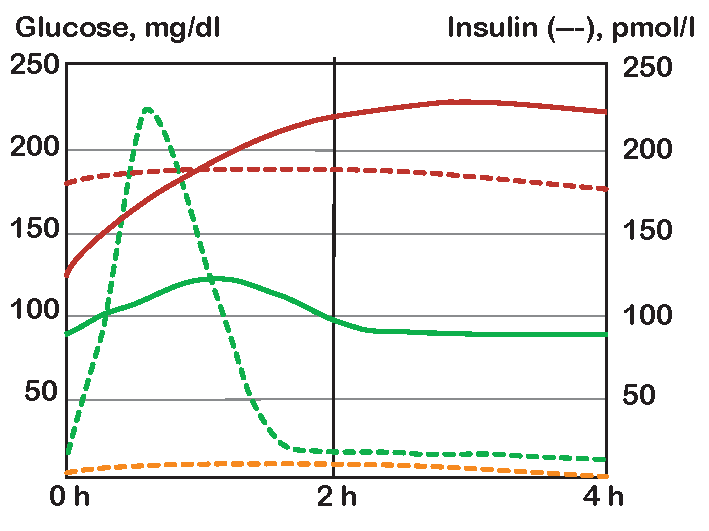
\includegraphics{graphics/glucoseTolerance.pdf}
\caption{Glucose tolerance test: A typical healthy patient has a very low fasting insulin level (dashed green line) and a high transient response to regulate a glucose intake a 0 hours. A healthy patient is able stabilize lower glucose level within 2 hours after glucose intake (green line). The insulin level of an untreated Type-2 patient (red dashed line) is already elevated and no further compensation is possible. The glucose level (red line) will stabilize. Yellow dashed line represent a Type-1 patient with almost no endogenous insulin production, if untreated glucose levels would exceed the ranges this axis. Figure is reproduced by redrawing and combining illustrations from \cite{silverthorn2010human,caumo2004first}}
\end{figure}

Type-2 accounts for the most incidents of diabetes and is strongly associated with lack of physical exercise, being overweight and an unfavorable diet. Other risk factors are age and genetic predispositions. Type-2 diabetes is not only a problem in industrialized countries.  World-wide 380 million people are estimated to have diabetes world wide and attributable to 15\% of deaths. \cite{aguiree2013idf}.

[alcohol][smoking][citer anden diabetes artikel med compliance?]

Intensive anti-diabetic therapy is important to avoid or delay myocardial infarct, micro vascular diseases and kidney related complications \cite{holman,boussageon2011effect,gaede2008effect}. Having a chronic elevated high blood glucose is simply very unhealthy long-term. As the type-2 diabetes progress glyceamic control is not achievable with a single oral agent such metformin or sulfonylurea. Injectable agents as insulin will inevitable be considered as the disease stage progress. Inconvenience and patient compliance are the main factors for not achieving the clinical recommendations for blood glucose control in insulin treatment of type II diabetes patients. To initiate injectable insulin therapy is a psychological barrier for Type-2 patients and a cause of worrying \cite{korytkowski2002oral}. Neverthelses insulin therapy will eventually become the outcome for most Type-2 patients. From early onset type-2 patients still have the ability to regulate blood sugar to some level and strict hourly control is not needed. In two groups group of 24,000 and 10,000 patients of seniors aged 60-69 (where), the former group was diagnosed with type-2 diabetes within last 9 years and the ladder group has been diagnosed for more than 9 year. When recently diagnosed, patients are prescribed oral hypoglycaemic agents (OHA). 50\% of early diagnosed received metformin and/or sulfonylurea. Only 7.5\% received insulin treatment. In contrary, for patients diagnosed for more than 9 years fully 65\% are ordinated treatments based on injectable insulin \cite{Elbert2014rates}. Thus a typical type-2 diabetes disease progression will start with fairly convenient once a day tablets, mildly lowering glucose. With time, more potent insulin is needed to obtain sufficient blood glucose control. The disease will progress from the needed treatment is only complimenting the blood sugar regulating mechanisms of the body itself, to the insulin therapy will be the main regulation of blood glucose.

Compliance is the extent of which the patient uses the medicine as prescribed by the physician. Especially for short acting injectable insulins, daily awareness and monitoring of blood glucose and having injectable insulin pens refrigerated may be a huge requirement for the patient. Type-1 patients who came to master these skills early in life, are likely to have a much higher compliance.

Simply, the patient must learn to live by a fairly complex treatment regimen late in life. Compliance for only oral agents can be as low is 50\% after six months \cite{garcia2013adherence}. As the disease progress, patients are expected to need injectable insulin at some point. In a study 50\% of insulin-naive patients percieved injectable insulin inititaion as a failure. In a study, of those patients who did not comply to an treatment regime with injectable insulin, the most common reasons given were planing to improve healthy behavior (25\%), fear of injection (13\%), negative impact on work (9\%), concerns on long-term medication (9\%), inconvenience (6\%), and not believing insulin was necessary (6\%). Despite the available various available anti diabetic agents for various stages of type-2, it is indicated that less than 50\% of patients achieve the aimed glucose control recommended and around two-thirds will die prematurely of cardiovascular disease \cite{garcia2013adherence}. In contrary it is argued that current injection pens actually have improved comfort for insulin injection so much, that needle fobia alone is not at strong argument for developing oral insulin formulations \cite{maher2014formulation}.

The possible introduction of oral insulin may provide a mid-way solution especially for Type-2 patients where other oral agents no longer are potent enough, yet with the same ease of administration as oral agents. Thus oral insulin may prolong the time the patient can regulate blood sugar without injectable insulin and perhaps improve compliance.

\section{Drug Development Challanges of Oral Insulin}

Oral formulations of insulin is not an obviously great idea. From natures side, an organism tend not take up any foreign substances, and certainly not foreign proteins or peptides. Proteins taken up are likely produced by foreign species, and therefore have been created to serve independent purposes, that not necessarily are in alignment with the survival of the organism.
Likewise, the human body have a series of barriers in the gastrointestinal tract before proteins such as insulin, reach systemic circulation. Figure \cref{intro_glucoseTolerance} illustrates the upper gastrointestinal tract and the barriers for insulin. Normal protein absorption, or more correctly amino acid absorption, starts in the stomach with the enzyme pepsin cleaving protein amide-bonds next to lipophilic/aromatic amino acids. Insulin formulations are simply protected towards pepsin and acidic hydrolysis with an acid insoluble tablet coating. The coating is made of polymers with pH-dependent solubility. Acidic side groups will deprotonate only under neutral pH and increase the solubility of otherwise lipophilic polymers. \cite{carino1999oral,gabor2010improving}. Most coatings are designed to dissolve at pH > 5.5 \cite{maher2014formulation}.
The insulin producing gland, pancreas, is also very central to the gastro intestinal digestion. The sphincther, the opening muscle of the stomach, forward some of the stomach content to the upper duodenum. The pancreas will secrete to the pancreatic duct the alkaline carbonate to neutralize the hydrochloric stomach acid. Pepsin is deactivated by neutral pH, while neutral acting trypsin and chymotrypsin are released from the pancreas as well. Depending on thickness and acid groups of coating polymer, the tablet/capsule will start dissolving immediately in the duodenum and jejunum or as late as in the colon.

The stomach empties approximately only every 50-120 minutes during fasting and even longer for diabetic patient \cite{silverthorn2010human,corvilain1995effect,gabor2010improving}, the accuracy of timing the dose are not likely to match injectable insulin. Therefore, oral insulin is not likely to replace fast acting well timed doses of injectables used by type-1 diabetics in connection with meals. Oral insulin is most likely to replace longer acting insulins where the exact onset of action is of less concern.

The luminal enzyme activity by trypsin and chymotrypsin will likely inactivate released insulin in less than 5-15 minutes \cite{welling2014citric}.

Presently several oral insulin formulation are clinical phase two and three. These formulation can rely on protein backbone modification to make insulin intrinsic more stable to enzymatic degradation, absorption enhancers, enzyme inhibitors (soybean, citric acid) and micro/nano-encapsulated carriers \cite{aguirre2016current}. Oral delivery of other peptides such as glukagon-like peptide-1 (GLP-1) analogues, salmon calcitonin, octreotide (somatostain agonist), parathyroid hormone are also in clinical development in 2012.

Peptide API's in oral formulations targeting systemic circulation, that have been approved by FDA or EMA are Cyclosporin (MW 1200) Desmopressin (MW 1100), Taltirelin Taltirelin  (MW 500) and glutathione (MW 300). \cite{aguirre2016current}. The reason these four API have been successfully introduced to market before insulin are likely in part the significant smaller size than monomere insulin (MW 6000) and these peptides can therefore permeate the epithelial barrier more easily. 


With the current formulation technology it is only possible to do so much. \quote{"The selection of a suitable peptide for oral formulation is, therefore, a key commercial decision. For example, selecting a complex, high molecular weight (MW), narrow therapeutic index peptide, manufactured by a costly recombinant approach, requiring multiple daily oral administrations would be problematic."}

Maher \textit{et al} points out that oral peptide delivery  for decades have been in its infancy and that we cannot suddenly deliver any type of peptide. In fact the current achievements are more attributable to the biotechnological advances allowing modification of the peptide and cheap production.

Pharmacokinetic profiles. Treatment with injectable peptides such as insulin, GLP-1 and growth hormone have become more convenient the last decades, as the intrinsic endogenous hormone have been modified to increase the half-life. Hereby, patients treated with a constant level of hormone, only have to inject themselves daily or even weekly. Oral peptides formulations at first will likely be attempted switches from their prenatally-marketed counterparts \cite{maher2014formulation}. As only a couple of percentages of peptide is likely absorbed the relative variation of absorption are potentially very high \cite{gabor2010improving}. A dosing interval significantly shorter than the half-life of the drug is a classic method for maintaining a relatively constant drug concentration within the therapeutic window \cite{tozer2006introduction}.

Analogues with enzymatic stability is also required. Co-formulation of soy-bean enzyme inhibitors \cite{fujii1985promoting}, covalent peptide protecters (SNAC) \cite{bruno2013basics}, pH lowering \cite{welling2014citric} can only lower degradation 2 to 5-fold. Designing stable analogues is also needed to obtain sufficient stability. PEGylation, cyclization and modification of back-bone structure are know approaches to increase intrinsic peptide analogue stability \cite{bruno2013basics}.

Thirdly peptide or proteins have to pass the epithelial barrier. Insulin (MW 6000 D) is likely near the upper limit of the size. For Octertide, it was possible to remove select a small part of peptide still retaining activity \cite{aguiree2013idf}. 

Fatty acids C8 to C12 have been to open tight junction between epithelial cells and mildly perturb the phospholipid membrane of the epithelials cells. There have been an extensive research {cite also brayden, c10, CMC} \cite{bruno2013basics} uncovering how C10 regulate calcium levels, and phosphyrolation cascades of the epithelial cells leading to opening of TJ. Nontheless, inorder to obtain a suffcient response C10 have to be presented on intestinal lumen in concentrations close to the critical micelle contration (which is) where the perturbing effect on phospholipid membrane sets in \cite{bruno2013basics}. No specific technology increasing protein absorption significantly have emerged from the C10-Calcium-TJ-theory. In practice fatty acids are surfactants, and most surfactants will destabilize the epithelial membrane and promote peptide absorption. The important part is how wide are the therapeutic window, potency versus toxicity and are these surfactant sufficiently soluble. Biological effects such as the C10-Calcium-TJ theory may render one surfactant slightly more or less potent and such effect would be difficult to predict, see section (modelling assumptions). The working hypothesis of this thesis is that central properties of surfactants are fairly possible to predict as they arise from non-complex physical phenomenas, and new absorption enhancers could be discovered simply from the expected structure.

Other solid state surfactant like enhancers tested for absorption enhancement. In common these enhancers all have a mono acyl chain typically from 8 to 16 carbon atoms. Other groups surfactant enhancers are the acyl-carnitines, acyl-cholates\cite{lee2000oral}, phosphocholines\cite{liu1999dodecylphosphocholine}, acyl-maltosides \cite{petersen2013colonic} and acyl sulphate \cite{anderberg1993epithelial}.

\begin{figure}[h]

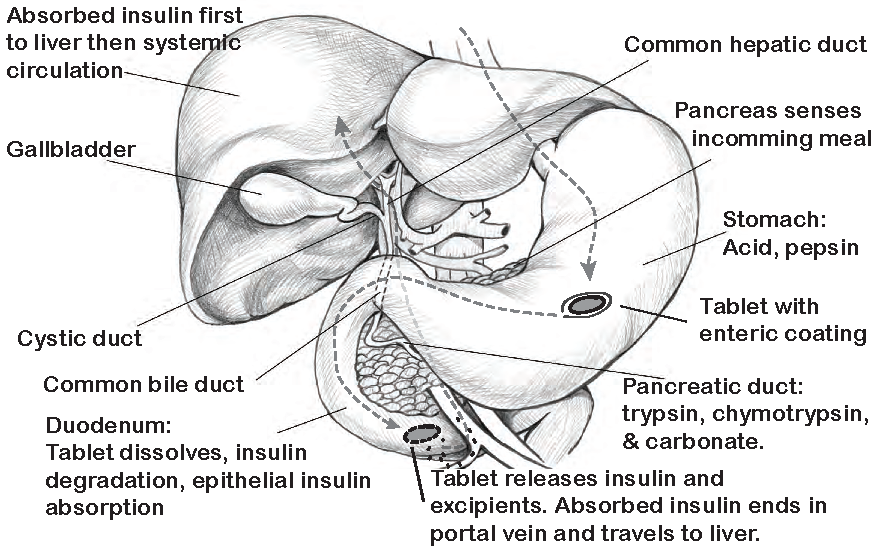
\includegraphics{graphics/intro_anatomy2.pdf}
\caption{(1) Tablet coating protects against acidic hydrolysis and pepsin. (2) Release of basic carbonate, bile, trypsin and chymotrypsin. Pepsin is inactivated at neutral pH. Bile interfere with surfactant like absorption enhancers. (3) Tablet dissolves. Lipophilic absorption enhancers will slow down insulin release and allow trypsin and chymotrypsin to inactivate all insulin before absorption. (4) Insulin permeates duodenal and jenunal epithelia facilitated by absorption enhancers. Illustration kindly provided for public use by NIH: National Institute of Diabetes and Digestive and Kidney Diseases. \url{https://catalog.niddk.nih.gov/imagelibrary/detail.cfm?id=148} Original captions modified.}
\label{intro_glucoseTolerance}
\end{figure}

\section{Studies to test peptide absorption}
Studies to test peptide absorption ranging from early proof-of-concept development to clinical trials late every are listed in Figure \ref{typeOfExperiment}. Beyond this list focusing on peptide absorption studies, also dedicated studies of \textit{in vitro} dissolution, peptide stability and toxicology would also be required.

mention low variance and bioavailabity are the goals.
introduce a 3-link chain model, dissolution, stability, permeation. 
membran transport/elctrical resistnace image?

In preclinical development, studies are formally segregated in two categories the \textit{ex vivo} outside the living and the \textit{in vivo} inside the living organism. Often \textit{in vivo} refer to animal studies, not human. The term \textit{in vitro}, in reagent glass, is used instead of \textit{ex vivo}. Speaking of \textit{in silico}, in silicium, is used for computer models. One may feel the latin buzzword terminology has been overly used to a point not \textit{in}. Further there are clinical trials in human. It is obviously sensible to test many new analogues in fairly inexpensive and fast studies. There are three main properties of oral formulations to optimize these are epithelial permeability, solubility and enzymatic stability. Most medical research observing and generalizing causal mechanisms. Where clinical trials can be very representative for the intended population of patients, it is difficult to learn exactly why a therapy elicited no positive result, there are multiple steps of failure and almost only the outcome percentage insulin absorbed into systemic circulation, the \% bioavailability, can be observed. Negative confirmation is important to narrow in what part of a therapy is essential for a positive outcome. Ethical considerations limit clinical trials to prescribe therapies to patients in conflict with their best self interest. With \textit{in vivo} studies it is possible to test treatments as long as the animal suffering as kept minimal. Still the gastro-intestinal tract are a complicated machinery and it is not possible to control or measure every aspect the peptide absorption process. Moreover other sources of variance such as the individual variance in animal physiology may introduce noise into measurements, therefore making step-wise incremental optimization of formulation difficult. When incremental formulation changes do not yield significant change of bio-availability. The lab bench \textit{in vitro} experiments offers close to full control of the experiment conditions. These experiments are often fast and or of low cost, while the reproducibility and statistical power are high. From a modeling perspective a larger set observations number is needed, especially for non-linear machine learning, to be introduced in section \ref{some section} and observations is assumed to be drawn independently. Therefore to get hands on \textit{in vitro} data is more easy. We only expect models built on data generated from \textit{in vitro} experiments, to reflect the   experiment. With a hopefully sufficient theoretical understanding of peptide absorption and the various biases of the \textit{in vitro} experiments, we can hope proving useful predictions and identify potential causal relationships between formulation and outcome.

\subsection{Caco-2 monolayers}
Caco-2 monolayers have been a standard screening method for intestinal drug permeability. The Caco-2 permeation model, as other permeation models, concist of a donor chamber, a epithelial barrier and a reciever chamber. Caco-2 monolayers are colonic human cancer cells, which makes more prolific. When seeded on a 2 cm in diameter micro porous filter on a 12-well plate, the Caco-2 cell line will grow and form a epithelial monolayer. A typical test will use 4 monolayers per tested treatment and the study is to be repeated on a different day. During the test, the nutrient reach DDEM media is replaced with minimal buffer solution. The buffer solution only contain Calicum, potassium and sodium, some acid/base buffer and phosphate. These ions maintain isotonicity and a normal electrical membrane that many active membrane transporter receptors rely on. Within standard drug development of small molecules. A low permeability result would likely lead discarding the given analogue , as it easier to find a new analogue with a favorable permeability. To use Caco-2 monolayers to test absorption enhancers for oral peptide delivery make just a small part of the use of Caco-2 monolayers. Here the permeability of insulin is already low, and may be increased by a given absorption enhancer. For surfactant enhancers at high concentration the monolayer can become completely disrupted and a low concentration, no useful effect is observed.

\subsection{Measuring permeability}
To estimate how potent an enhancer is, two permeation markers have been used, these are human insulin and radio labeled mannitol. Mannitol, approximately being as hydrophilic as glucose, is thought to only be taken up by a trancellular pathway through the tight-junctions \cite{anderberg1992epithelial,artursson1994effect}. Mannitol is neither taken up by active transport as glucose would be. Likewise, trans epithelial electrical resistance (TEER) can measure how open the paracellular tight junctions are, as the junction cross sectional area is approximately proportional to the conductivity, inverse resistance. TEER the easiest non-invasive measurement. Lowering the epthelial resistance e.g. 50\% with a absorption enhancer will likely translate to a (?-fold increase) of permeability of both mannitol and insulin. FITC-dextran 4000 dalton (FD4) is a florescent labeled sugar polymer of similar hydrophilicity and size as insulin. FD4 can replace insulin as transport marker with no enzymatic cleavage.

\begin{figure}[h]
\label{devel_typeOf}
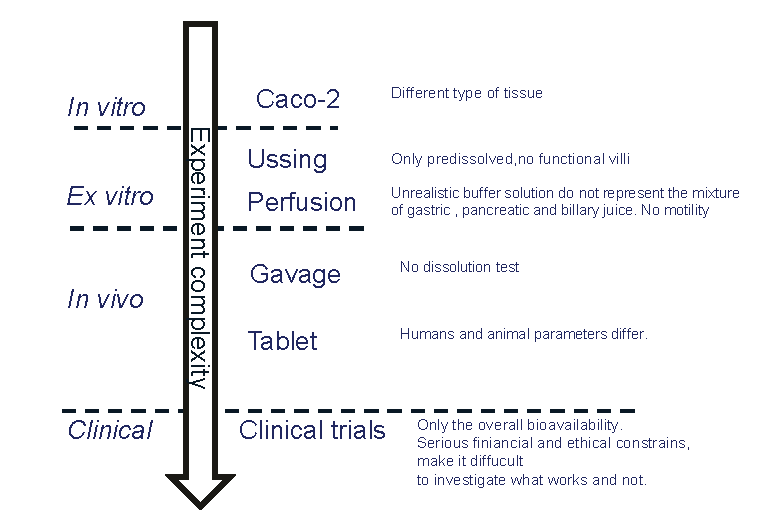
\includegraphics{graphics/typeOfExperiments.pdf}
\caption{Schematic overview of types of experiments ranging from Caco-2 to clinical. Simple experiments to not accurately simulate the actual process, and there will be a number of biases which must not be over interpreted.}
\end{figure}


\subsection{Calculating permeability}
Gradient driven diffusion of mannitol, FD-4 and insulin across the epithelial barrier is a first order process where the transport per time is proportional to the concentration gradient $C_i$ ($mol/L$). Only a few percent of the total amount of transport marker will permeate the barrier and therefore will $C_i$ be approximately unchanged throughout the experiment. Hereby becomes the apparent permeability $P_{app}$ proportional to the transport rate or flux $J$ ($mol/s$) which is usually estimated by sampling the reciever basolateral side 4 to 6 times. When plotting reciever concentration versus time, a fitted ordinary least squares slope is used as the overall transport rate through out the experiment. Permeability is corrected for the actual dimensions of the diffusion chamber. The flux $J$ is expected to be proportional to the difussion area $A$ (cm$^2$).  Therefore the apparent permeability is written caluculated as

$P_{app} = J/A / C_i \quad .$

The tight junctions are in theory water filled channels with a given conductance solute. When tight junction are widened, the cross-sectional area of tight-junction per area tissue is changed. As marker transport is driven by a concentration difference, the electrical charge transport rate, the electrical current $A_{e}$ (Ampere $A_c$), is driven by an electrical potential difference $U$ (Voltage V). The tissue conductivity $S$ corrected for area tissue $S_A = S/A$, is the equivalent to $P_{app}$. The $S_A$ is the inverse of the resistance $R$ multiplied by tissue area (Ohm cm2)

$frac{1}{RA} = S_A = A_e/A / U \quad$

To summarize both $P_app$ and inverse TEER both describe how readily a flux of either molecules or ions are driven through the epithelial barrier by respectively a concentration gradient electrical potential gradient. $P_app$ is measured by maintaining a constant concentration gradient determining the molecule flux. TEER is either measured with voltage or current clamping. To measure TEER with voltage clamping is to control the electrical gradient (potential difference) with electrodes and measuring the actual current. Current clamping is oppositely to drive a specied flux of ions (current) through the epithelial barrier and record the electrical gradient. As the tissue itself have an constant ion transport. TEER reflects the intrinsic permeability of the monolayers. For direct measurement of permeability of a given drug molecule, TEER is mainly used to check barrier integrity. For measuring the potency of permeation enhancers to increase permeability, TEER can be used as indicator hereof. To directly measure the permeation of insulin would be preferable, but more slow, expensive and unlikely to find in already published results.

\begin{figure}[h]
\label{devel_fassif}
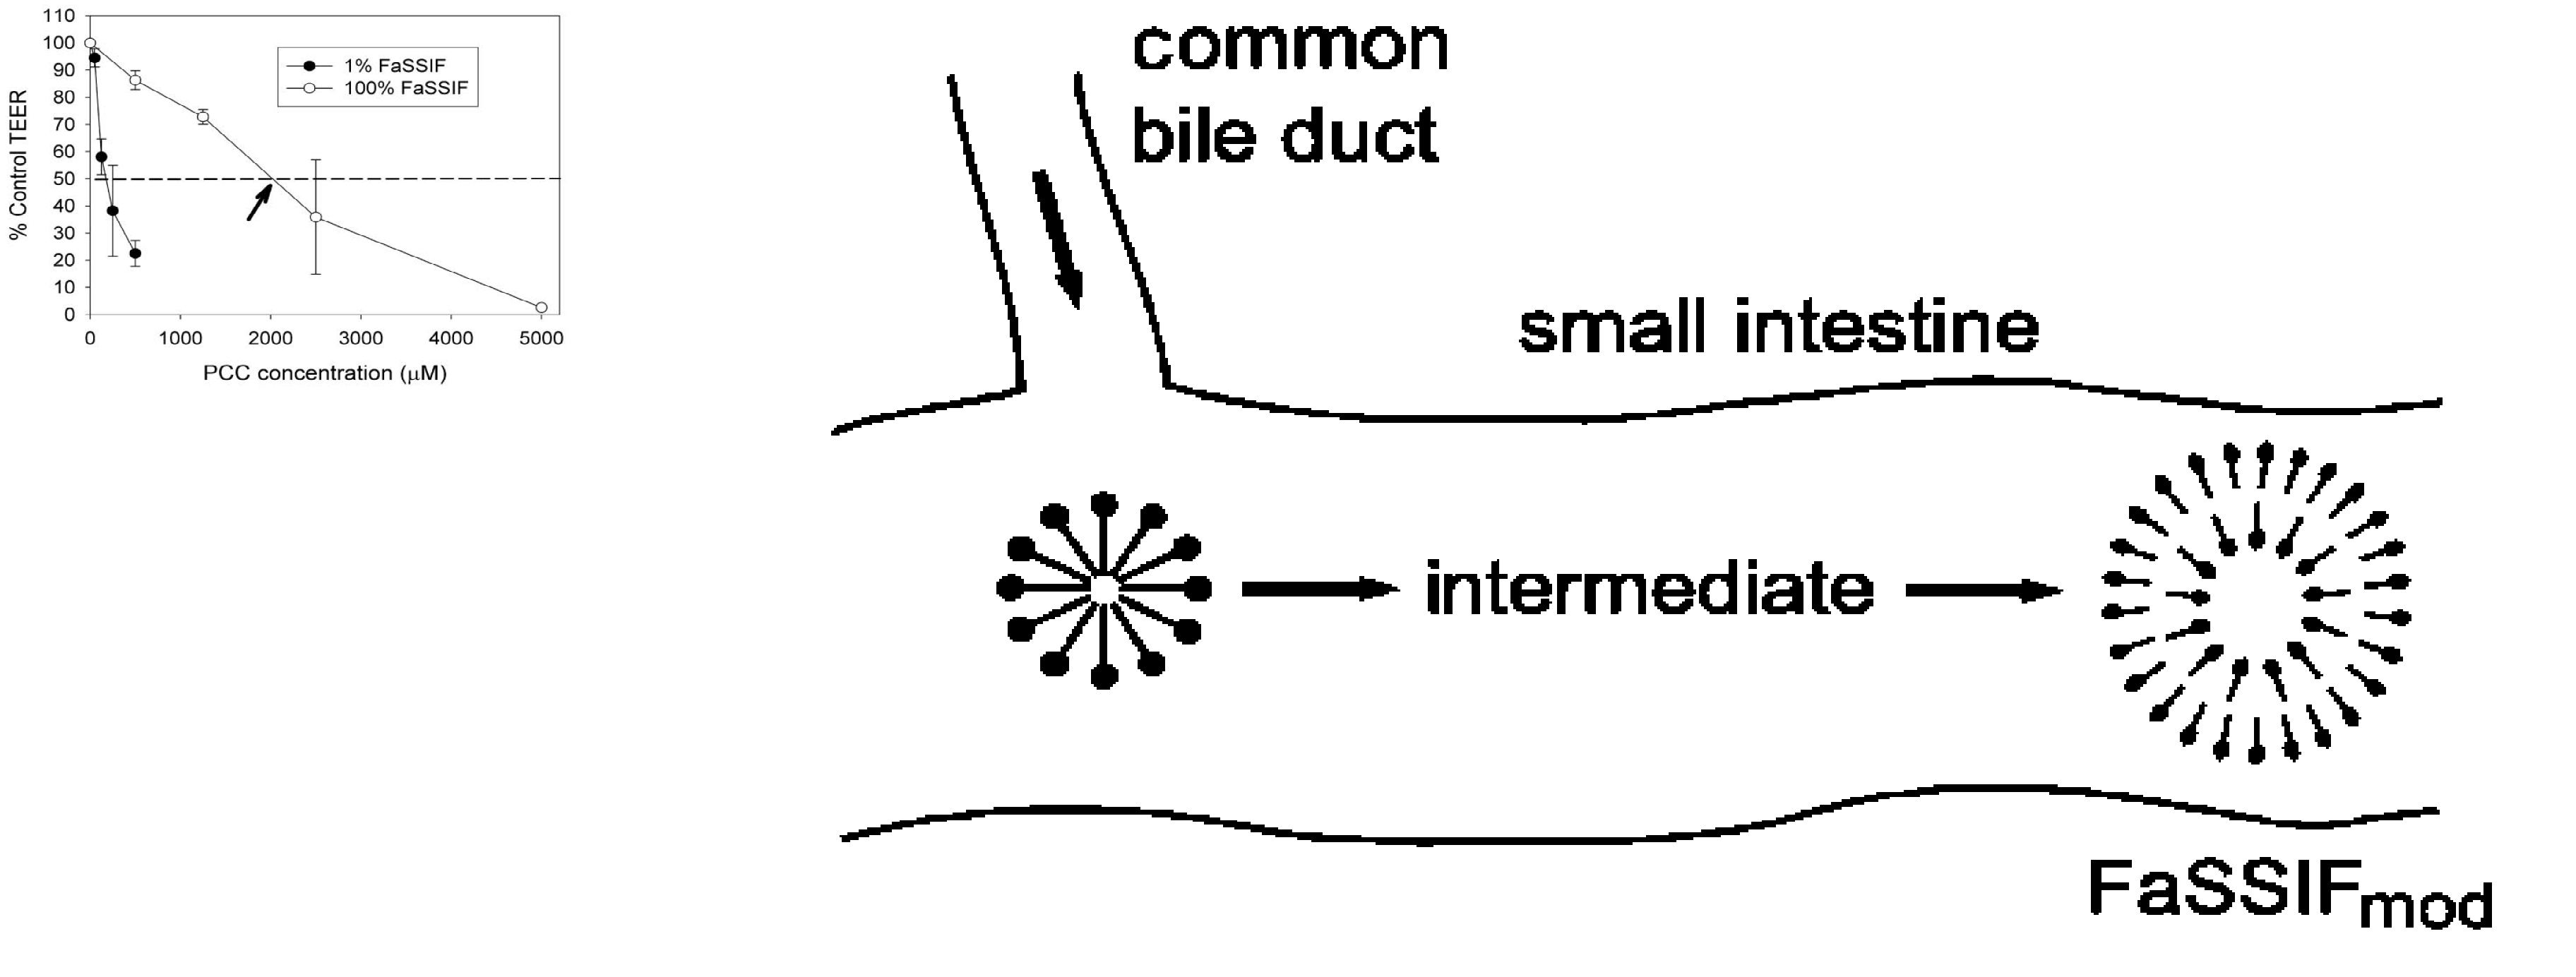
\includegraphics{graphics/devel_Fasssif_PCC2.png}
\caption{Single figures copied from \cite{tippin2008biorelevant,nawroth2011liposome} to illustrate why the potency of lipophilic permeation enhancers are likely overestimated in in-vitro studies using surfactant free buffers. Palmitoyl carnitine was found by Tippin \textit{et al} to be 12 times less potent in a Fassif buffer with Taurocholate and lechitine an EC$_{50}$}
\end{figure}


